{\color{mypink}
\subsection{Definition~\ref{def-stab--probing-nfs} implies definition \ref{def-stab-ra--probing-nfs}}

We have introduced two different definitions of filter stability in section~\ref{ssec-def-stab--probing-nfs}. Definition~\ref{def-stab--probing-nfs} is used for the numerical computations in this chapter while the other definition~\ref{def-stab-ra--probing-nfs} is a commonly used definition using the notion of weak convergence. In this appendix, we prove that~\ref{def-stab--probing-nfs} is stronger in the sense that it implies the other.
}
\begin{thm} Let $(M, d)$ be a compact metric space and $\{\alpha_n\}, \{\beta_n\}$ be sequences of random probability measures on $M$ with finite first and second moments and 
\begin{align}
    \lim_{n\to\infty}\mathbb E[D(\alpha_n, \beta_n)] = 0 \,,
\end{align}
where $D = W_1$ or $W_2$. Then for all globally Lipschitz functions $f: M \to \mathbb R$ we have
\begin{align}
    \lim_{n\to\infty}\mathbb E\left[\left|\int_M f\,d\alpha_n -\int_M f\,d\beta_n\right|\right] = 0 \,.
\label{eq-fconv--probing-nfs} \end{align}

\begin{proof}
Let $S=\{f:M\to\mathbb R:\rm{Lip}(f)\le 1\}$ be the set of Lipschitz functions with Lipschitz constant not greater than 1.
If $f\in S$, by Kantorovich-Rubinstein duality we have,
\begin{align}
    \mathbb E\left[\left|\int_M f\,d\alpha_n -\int_M f\,d\beta_n\right|\right] \le 
    \mathbb E\left[\sup_{g\in S}\left|\int_M g\,d\alpha_n -\int_M g\,d\beta_n\right|\right]=\mathbb E[W_1(\alpha_n, \beta_n)] \,,\label{eq:con-KR--probing-nfs}
\end{align}
which proves the assertion for the case $D=W_1$ for $f \in S$. For $D=W_2$, recall that for two measures $\mu, \nu$ on $M$ with finite first and second moments, 
\begin{align}
    W_p(\mu, \nu)^p = \inf_{\mathbb S}\mathbb E[d(X, Y)^p] \,, \label{eq:Wp-defn--probing-nfs}
\end{align}
where $\mathbb S = \{\pi: \pi \text{ is the joint distribution of } X, Y \text{ with marginals  } \mu, \nu \text{ respectively}\}$. Therefore,
\begin{align}
    W_1(\mu, \nu)^2 &= \left(\inf_{\mathbb S}\mathbb E[d(X, Y)]\right)^2=\inf_{\mathbb S}\mathbb E[d(X, Y)]^2 \le \inf_{\mathbb S}\mathbb E[d(X, Y)^2], \quad\text{[by Jensen's inequality]}\\
    &\le W_2(\mu, \nu)^2,\quad\text{[by } \eqref{eq:Wp-defn--probing-nfs}] \label{eq:Wp-ineq--probing-nfs}
\end{align}
Combining \eqref{eq:con-KR--probing-nfs} and \eqref{eq:Wp-ineq--probing-nfs}, we immediately see that the assertion is true for the case $D = W_2$ for $f \in S$.

Now pick a function $\tilde{f}: M\to\mathbb R$ with $\text{Lip} (\tilde f)\le K$ for some $K>0$. Define $f=\frac{\tilde{f}}{K}$. Clearly, $f\in S$ and therefore,
\begin{align}
    \lim_{n\to\infty}\mathbb E\left[\left|\int_M \tilde f\,d\alpha_n -\int_M \tilde f\,d\beta_n\right|\right] =K\lim_{n\to\infty}\mathbb E\left[\left|\int_M f\,d\alpha_n -\int_M f\,d\beta_n\right|\right] =0 \,, 
\end{align}\label{thm:lip--probing-nfs}
\end{proof}
\end{thm}

Theorem~\ref{thm:lip--probing-nfs} immediately yields the following stronger statement.
\begin{cor}Under identical conditions, \eqref{eq-fconv--probing-nfs} holds for any continuous $f:M\to\mathbb R$.

\begin{proof}

Note that real-valued, continuous functions on $M$ are uniform limits of locally Lipschitz functions on $M$. Since $M$ is compact and locally Lipschitz functions on compact metric spaces are globally Lipschitz, real-valued, continuous  functions on $M$ are uniform limits of globally Lipschitz functions on $M$. 

Let $\alpha_n - \beta_n=\gamma_n$ for brevity and let $f$ be a real-valued, continuous function on $M$.
\begin{align}
    \left|\int_M f\,d\alpha_n - \int_M f\, d\beta_n\right| = \left|\int_M f\,d\gamma_n\right| = \left|\int_M f^+\,d\gamma_n^+ + \int_M f^-\,d\gamma_n^- - \int_M f^-\,d\gamma_n^+ - \int_M f^+\,d\gamma_n^-\right| \,,
\end{align}
where $+, -$ denote the positive and negative parts of $f$ and $\gamma_n$. We now consider the case when the last sum of four terms is positive. The other case when it is negative is very similar.

Pick sequences of non-negative globally Lipschitz functions $f^+_m\uparrow f^+$ and $f^-_m\uparrow f^-$. Then by using dominated convergence theorem and Fatou's Lemma, we see that
\begin{align}
    \mathbb E\left[\int_M f^+\,d\gamma_n^+\right] = \mathbb E\left[\lim_{m\to\infty}\int_M f^+_m\,d\gamma_n^+\right] \le \mathbb E\left[\liminf_{m\to\infty}\int_M f^+_m\,d\gamma_n^+\right] \le \liminf_{m\to\infty}\mathbb E\left[\int_M f^+_m\,d\gamma_n^+\right] \,.
    \label{eq:ineq1--probing-nfs}
\end{align}
Using very similar arguments for each of the four terms and adding the four inequalities, we see that 
\begin{align}
   \mathbb E\left[\left|\int_M f\,d\alpha_n - \int_M f\,d\beta_n\right|\right] \le \liminf_{m\to\infty}\mathbb E\left[\int_M f^+_m\,d\gamma_n^+\int_M f^-_m\,d\gamma_n^--\int_M f^-_m\,d\gamma_n^+-\int_M f^+_m\,d\gamma_n^-\right] \,. \label{eq:ineq-combo--probing-nfs}
\end{align}
Define, $f_m = f_m^+ - f_m^-$ which is globally Lipschitz since sum of globally Lipschitz functions are globally Lipschitz. Since the RHS of \eqref{eq:ineq-combo--probing-nfs} is non-negative, it must be equal to $\liminf_{m\to\infty}\mathbb E\left[\left|\int_M f_m\,d\gamma_n\right|\right]$. Therefore,
\begin{align}
    \mathbb E\left[\left|\int_M f\,d\alpha_n - \int_M f\,d\beta_n\right|\right]\le\liminf_{m\to\infty}\mathbb E\left[\left|\int_M f_m\,d\alpha_n - \int_M f_m\,d\beta_n\right|\right] \,.
\end{align}
Hence, given $\varepsilon > 0, \,\exists\, m_0$ such that $\forall \, m > m_0$, 
\begin{align}
\mathbb E\left[\left|\int_M f_m\,d\alpha_n - \int_M f_m\,d\beta_n\right|\right] > \mathbb E\left[\left|\int_M f\,d\alpha_n - \int_M f\,d\beta_n\right|\right] - \varepsilon \,.
\end{align}
Using theorem~\ref{thm:lip--probing-nfs}, we see that the limit $n \to \infty$ of LHS is $0$ which gives
\begin{align}
    & 0 \ge \lim_{n\to\infty}\mathbb E\left[\left|\int_M f\,d\alpha_n - \int_M f\,d\beta_n\right|\right] - \varepsilon \,.
\end{align}
Since $\varepsilon$ can be chosen arbitrarily, we have
\begin{align}
    \lim_{n\to\infty}\mathbb E\left[\left|\int_M f\,d\alpha_n - \int_M f\,d\beta_n\right|\right] = 0  \,.
\end{align}
\end{proof}
\label{cor:cts--probing-nfs}
\end{cor}

\begin{thm} Assume the filtering distributions $\hat\pi_n(\mu),\hat\pi_n(\nu)$ are supported on a compact subset of $\mathbb R^d$ and $D=W_2$ or $W_1$. If \eqref{eq-stablaw--probing-nfs} holds then so does \eqref{def-stab-sumith--probing-nfs}.
\begin{proof}
Direct consequence of corollary~\ref{cor:cts--probing-nfs}.
\end{proof}
\label{thm:strength--probing-nfs}
\end{thm}
{\color{mypink}\subsection{Convergence in $D_\varepsilon$ and $W_2$}\label{ssec-dw--probing-nfs}
\begin{thm} Suppose 
$\exists$ a sequence $p_k: \lim_{k\to\infty}p_k=0$ and $  a_{kn}:=\mathbb E[D_{p_k}(\alpha_n, \beta_n)]$ is monotone decreasing in $k$ or, 
$a_{kn} \ge a_{k+1,  n}\;\forall\; k, n$ where $\{\alpha_n\}, \{\beta_n\}$ are sequences of random measures. If for some $j$
\begin{align}
    \limsup_{n\to\infty}\mathbb E[D_{p_j}(\alpha_n, \beta_n)] \le \delta,
\end{align}
then
\begin{align}\limsup_{n\to\infty}\mathbb E[W_2 (\alpha_n, \beta_n)]\le\delta
\end{align}

\begin{proof}
Recall that $\lim_{k\to\infty}D_{p_k} (\alpha_n, \beta_n) = W_2 (\alpha_n, \beta_n)$, see for example, theorem $1$ in \cite{genevay2018learning}. By Fatou's lemma,
\begin{align}
    \limsup_{n\to\infty}\mathbb E[W_2 (\alpha_n, \beta_n) \le \limsup_{n\to\infty}\liminf_{k\to\infty}\mathbb E[D_{p_k}(\alpha_n, \beta_n))] \le  \limsup_{n\to\infty}\mathbb E[D_{p_j}(\alpha_n, \beta_n))]\le\delta
\end{align}
\end{proof}
\label{thm:w2-limsup-bound--probing-nfs}
\end{thm}
Theorem ~\ref{thm:w2-limsup-bound--probing-nfs} is helpful in discussing the convergence of measures in Wasserstein metric by looking at convergence in $D_\varepsilon$ for a fixed $\varepsilon$. The assumption about existence of a monotone decreasing subsequence is consistent with numerical experiments as shown in figure~\ref{fig:bpf-eps-all--probing-nfs}. Although Sinkhorn divergence is zero when we are comparing two identical distributions, while comparing two different samples from the same distribution we would expect a non-zero divergence which is why theorem~\ref{thm:w2-limsup-bound--probing-nfs}  is stated in terms of a non-zero bound $\delta$. We note that a more detailed discussion about the behaviour of this non-zero divergence can be found in section~IV.A in~\cite{mandal2021stability}. With increasing sample size this non-zero divergence approaches zero. For a detailed look at the theoretical sample-complexity of Sinkhorn divergence see chapter~$3$ of~\cite{genevay2019entropy}.
\begin{figure}
    \centering
    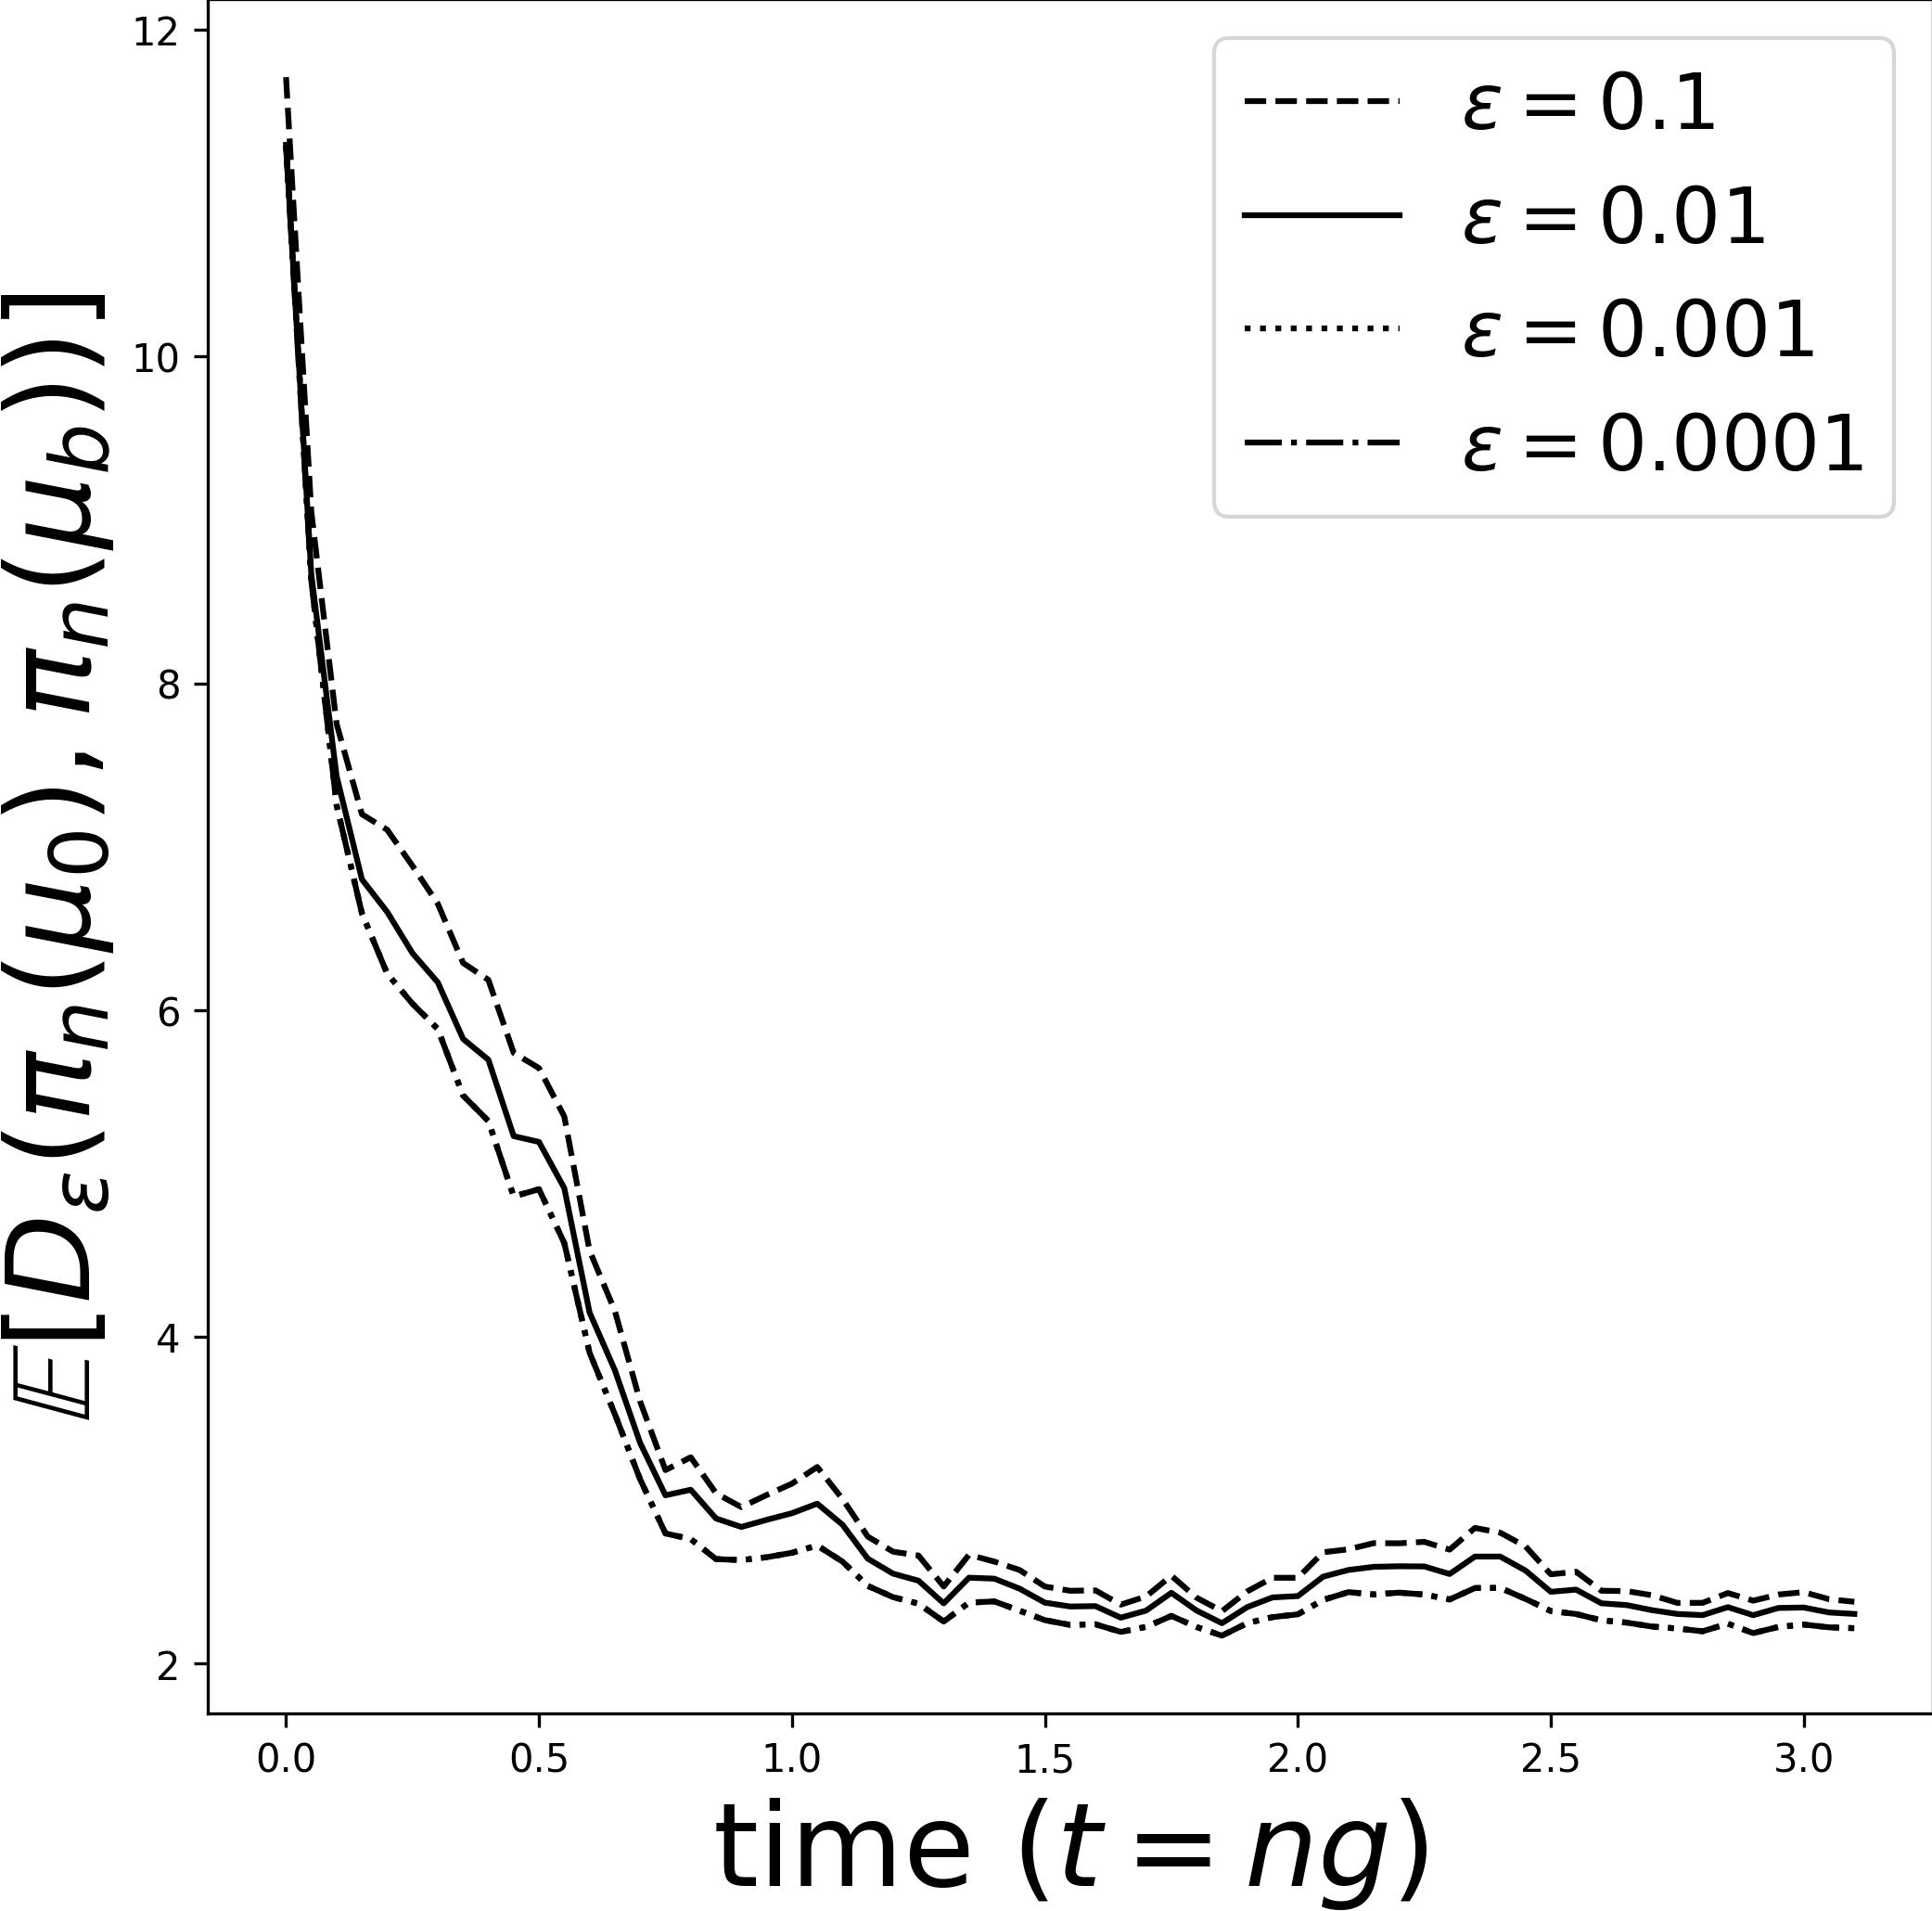
\includegraphics[scale=0.15]{stability/plots/plots-bpf-eps_all.jpg}
    \caption{Change in mean $D_\varepsilon$ with $\varepsilon$. The smallest two  $\varepsilon$ values produce identical mean lines. The filtering distributions are generated by particle filter for observation gap  $=0.05$ and observation covariance $=0.4$.}
    \label{fig:bpf-eps-all--probing-nfs}
\end{figure}
}

{\color{mypink}\subsection{Effect of varying the sample-size}\label{ssec-sample-size--probing-nfs}
We find that averaging over $10$ observation realizations (for the expectation in~\eqref{eq-stablaw--probing-nfs}) is sufficient for this study. To illustrate this, we repeated a representative experiment for a larger sample size  of $100$ and the resulting plots of the distance versus time for observation gap $g=0.05$ and $\sigma^2=0.4$ for the two filters are shown in figure~\ref{fig:obs-100--probing-nfs}. Comparing with the plots in first row, second column of the particle filter and EnKF results in figure~\ref{fig:bpf-enkf-fixed-ogap--probing-nfs}, we see that the results are qualitatively identical and quantitatively near-identical. Thus the choice of averaging over $10$ realizations suffices to capture the statistical features of the quantities we are studying.
\begin{figure}
    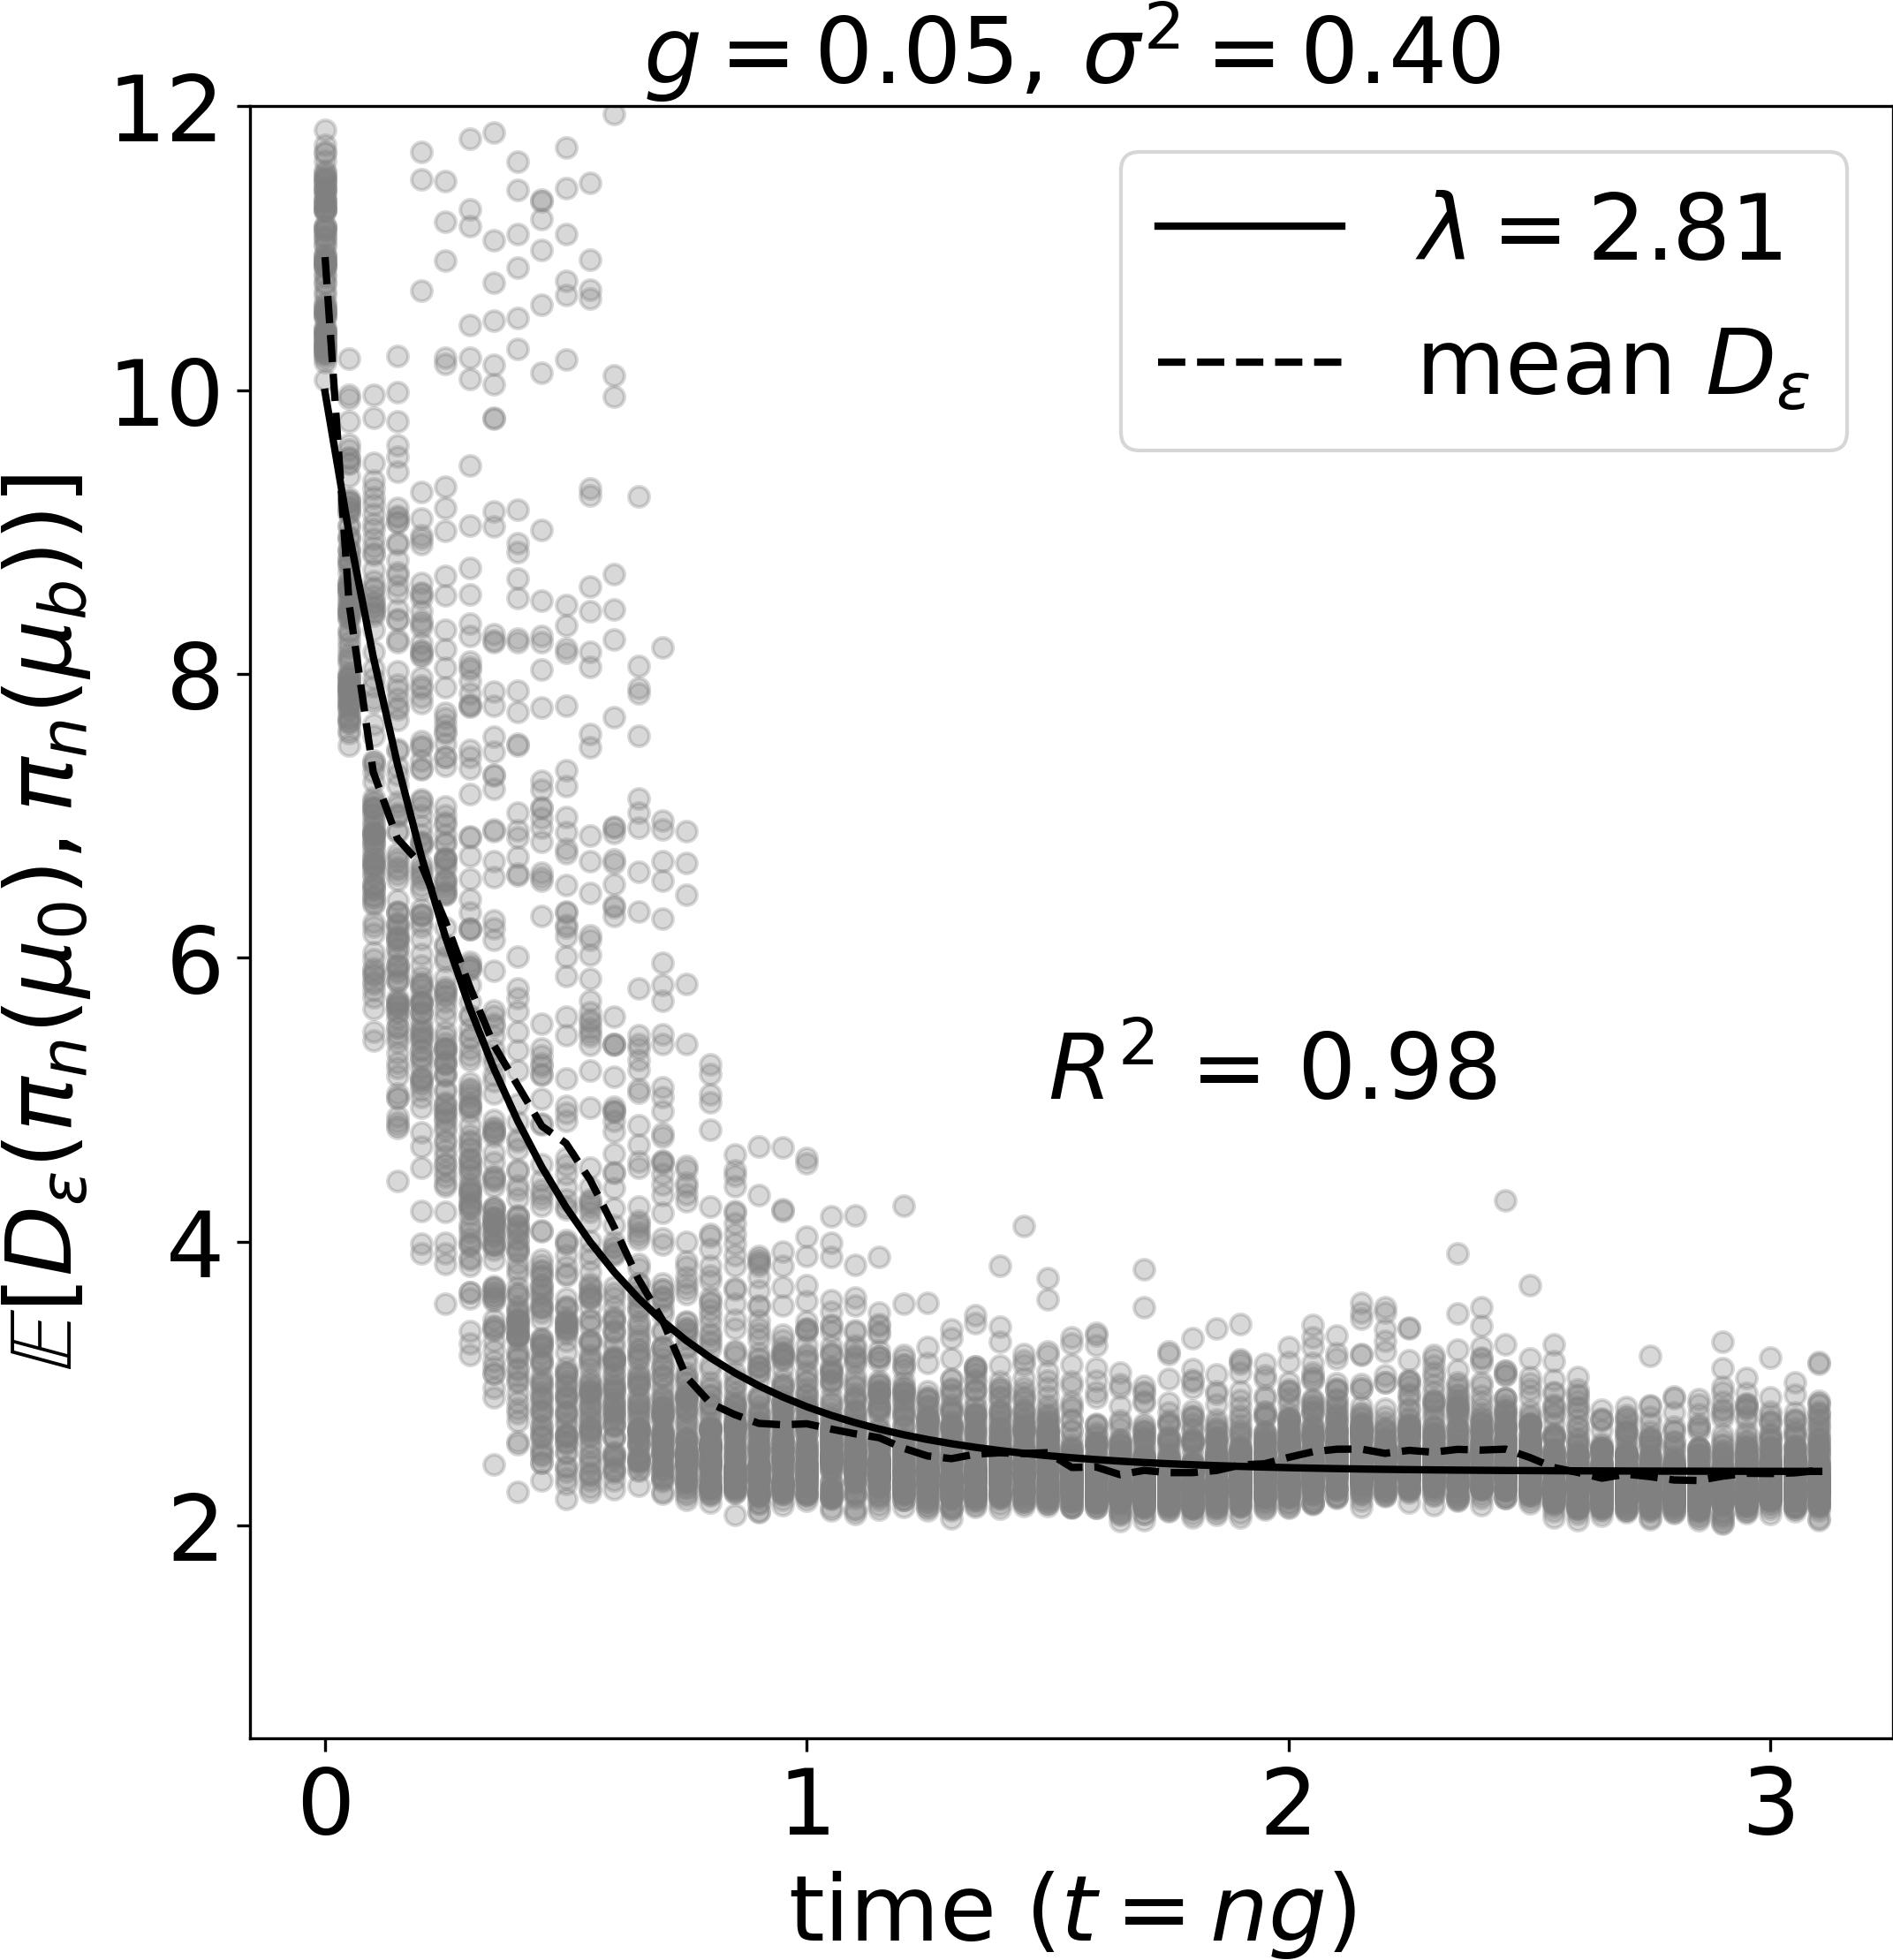
\includegraphics[scale=0.1]{stability/plots/plots-bpf-rate_obs_100.jpg}
    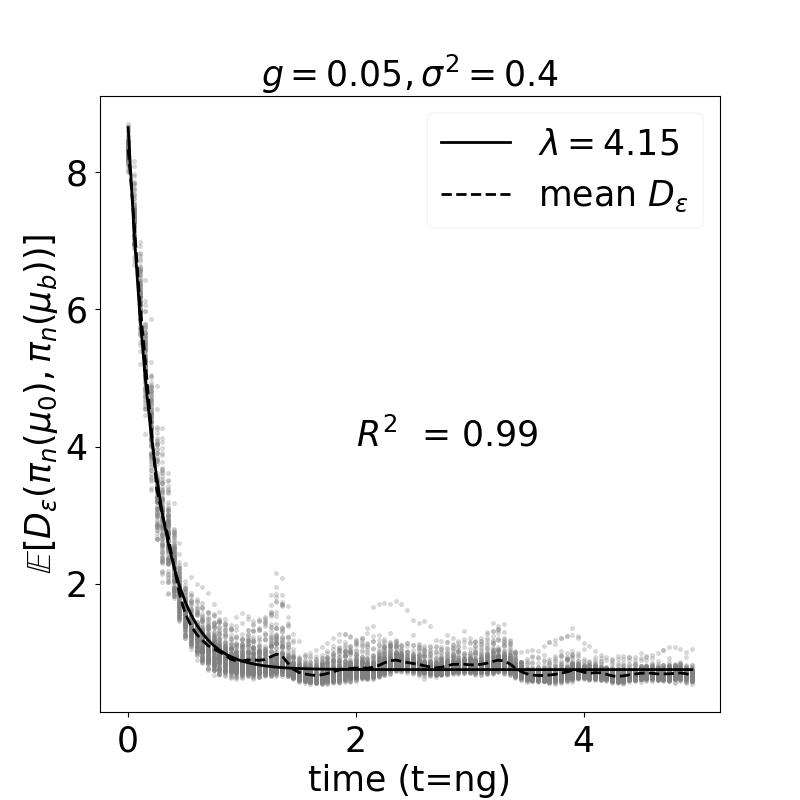
\includegraphics[scale=0.3]{stability/plots/plots-enkf-100_enkf.jpg}
    \caption{Mean $D_\varepsilon$ for $100$ observations for PF (left panel) and EnKF (right panel) with observation gap  $=0.05$ and observation covariance $=0.4$.}
    \label{fig:obs-100--probing-nfs}
\end{figure}
}



